% \documentclass{article}
\documentclass[11pt,a4paper]{exam}

\usepackage{exercices}
\usepackage{mdframed}
\usepackage{float}
\usepackage{siunitx}
\usepackage{tikz}

\usetikzlibrary{calc}
\usetikzlibrary{positioning}
\usetikzlibrary{arrows.meta}
\usetikzlibrary{decorations.pathmorphing}
\usetikzlibrary{angles, quotes}

\datehead{26 janvier 2023}
\qformat{{\large\bf\thequestion . \thequestiontitle.\hfill}}
\newcommand{\spacev}{\textcolor{white}{Du texte\\}}

\usepackage[utf8]{inputenc}
\usepackage{amsmath}
\usepackage{amsfonts}
\usepackage{graphicx}
\usepackage{bm}
\title{Exercice de mécanique 2022}
\date{Décembre 2022}
\author{Antoine C.D. Hoffmann}

\newcommand{\exACDH}{\bm e_x}
\newcommand{\eyACDH}{\bm e_y}
\newcommand{\ezACDH}{\bm e_z}
\newcommand{\erACDH}{\bm e_r}
\newcommand{\etACDH}{\bm e_\theta}
\newcommand{\noteACDH}[1]{\textit{Remarque: #1}}

\begin{document}

\section*{La tyrolienne}
%\titledquestion{La tyrolienne}



\begin{figure}
    \centering
    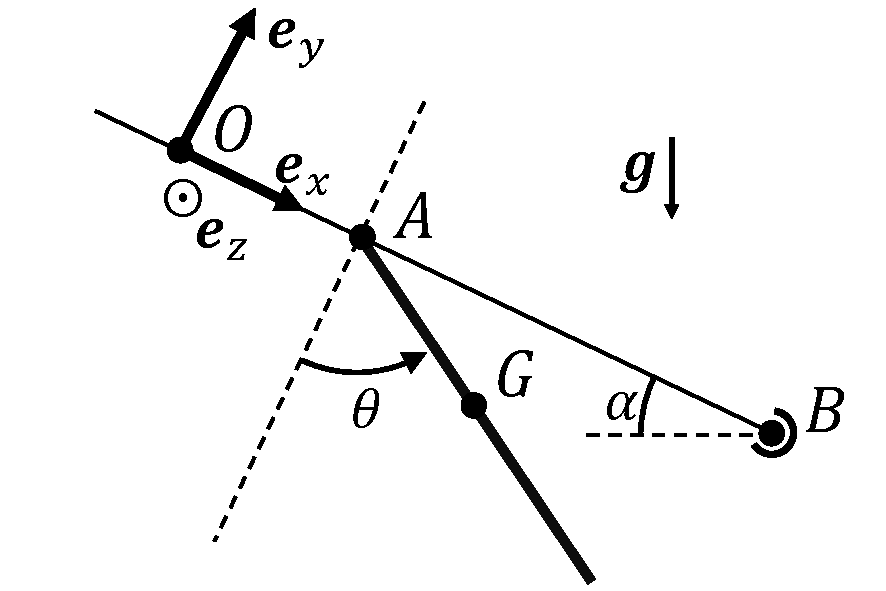
\includegraphics[width=0.55\linewidth]{ExoFig/tyr_schema.pdf}
\end{figure}
%% Enoncé
Une tyrolienne est modélisée par une barre indéformable, homogène, de masse $m$ et de longueur $2l$.
Le point d'attache de la barre $A$ est libre de glisser le long d'un câble rigide, incliné d'un angle $\alpha$ par rapport à l'horizontale. 
On dénote par $G$ le centre de masse de la barre et par $I_G$ le moment d'inertie de la barre selon un axe de rotation perpendiculaire à elle-même autour de ce point. 
On définit le repère cartésien $(\exACDH, \eyACDH, \ezACDH)$, centré au point $O$ placé sur le câble.
On détermine la position de la tyrolienne par la position du point d'attache $\overrightarrow{OA}=x_A(t) \exACDH$ et par l'angle $\theta(t)$ défini par rapport à un axe perpendiculaire au câble.
La gravité $\bm g$ agit vers le bas. On néglige tout effet de frottement et on suppose que la barre ne bouge que dans le plan du schéma.\\
Lorsque le point d'attache $A$ arrive au point $B$ situé à une distance $d$ de $O$ ($d=|\overrightarrow{OB}|$), un mécanisme empêche instantanément tout déplacement de $A$ mais laisse $\theta$ libre, c'est-à-dire que la barre reste libre de tourner autour du point $B$.
%
\begin{parts}
%%% PREMIERE PARTIE
\uplevel{On étudie d'abord le mouvement de la tyrolienne le long du câble avant son arrivée en $B$.\vspace{2.0mm}}
%%%%%%%%=========================================================================
\part{Lister les forces s'appliquant à la tyrolienne, les projeter sur le repère $(\exACDH, \eyACDH, \ezACDH)$ et appliquer la seconde loi de Newton.}
%\begin{solution}
    \par\vspace{2mm}
    Les forces en présence sont la gravité
    \begin{align}
        m\bm g &= mg\sin(\alpha) \exACDH - mg\cos(\alpha) \eyACDH
    \end{align}
    et la force de soutient normale au câble
    \begin{align}
        \bm N  = N \bm e_y.
    \end{align}
    
    Le théorème du centre de masse stipule que l'on peut appliquer la seconde loi de Newton en considérant chaque force appliquée sur la barre au centre de masse G.
    On obtient alors 
    \begin{align}
        m \bm a_G &= \sum \bm F \nonumber\\
        \Leftrightarrow m (\bm a'_G + \bm a_A) &= m\bm g + \bm N \label{eq:newtonCM}
    \end{align}
    o\`u $\bm a_G$ est l'accélération du centre de masse selon le référentiel d'inertie lié à $O$ et $\bm a'_G$ selon le référentiel accéléré lié à $A$. $\bm a_A$ est l'accélération relative du référentiel lié en $A$ par rapport au référentiel d'inertie.
    En utilisant le repère cartésien $(\exACDH,\eyACDH)$, on écrit la $\overrightarrow{OA}=x_A \exACDH$ et donc l'accélération $\bm a_A$ s'écrit
    \begin{equation}
        \bm a_A = \frac{\mathrm d^2}{\mathrm dt^2}\overrightarrow{OA}= \ddot x_A \exACDH.
    \end{equation}
    D'une manière similaire, l'accélération relative du centre de masse $\bm a'_G$ peut s'obtenir en dérivant deux fois la position du centre de masse dans le repère $(\exACDH,\eyACDH)$, i.e. $\overrightarrow{AG}=l\sin(\theta)\exACDH-l\cos(\theta)\eyACDH$.
    \begin{align}
        \bm a'_G &= \frac{\mathrm d^2}{\mathrm dt^2}\overrightarrow{AG}\nonumber\\
        &= \frac{\mathrm d}{\mathrm dt}\left[l\cos(\theta)\dot\theta \exACDH + l\sin(\theta)\dot\theta \eyACDH \right]\nonumber\\
        &= \left[l\cos(\theta)\ddot\theta  - l\sin(\theta)\dot\theta^2 \right]\exACDH +  \left[l\sin(\theta)\ddot\theta + l\cos(\theta)\dot\theta^2\right]\eyACDH
    \end{align}
    Ainsi, l'équation Eq. \eqref{eq:newtonCM} se développe selon $\exACDH$ et $\eyACDH$ en
    \begin{align}
    ml\ddot\theta\cos(\theta) - ml\dot\theta^2 \sin(\theta)  + m\ddot x_A &= m g \sin(\alpha)\label{eq:newton_ex}\\
    ml\ddot\theta\sin(\theta) +ml \dot\theta^2\cos(\theta) &= N - mg\cos(\alpha) \label{eq:newton_ey}.
    \end{align}
    
     \begin{figure}
         \centering
         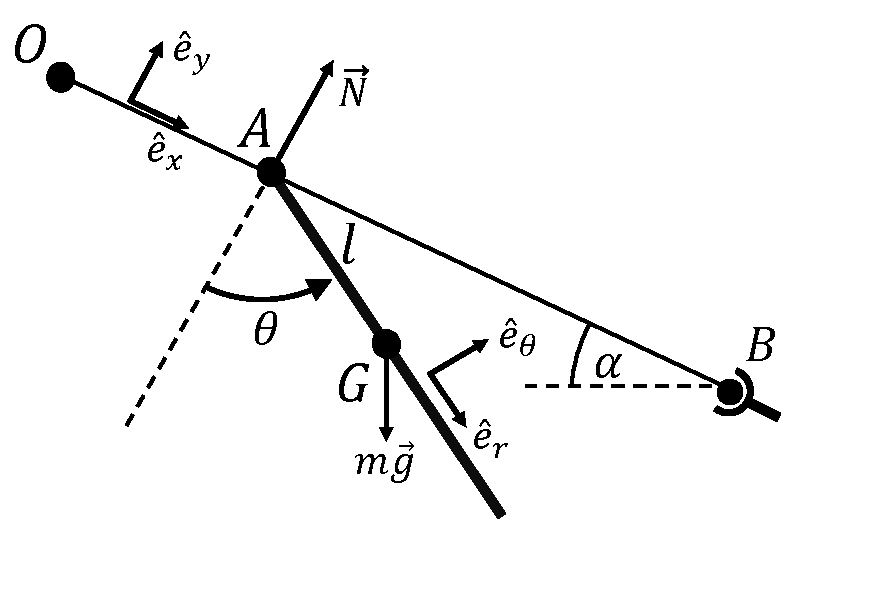
\includegraphics[width=0.5\linewidth]{ExoFig/tyr_schema_details.pdf}
         \caption{Schéma détaillé du problème}
         \label{fig:schema_details}
     \end{figure}
%\end{solution}

%%%%%%%%=========================================================================
\part{Appliquer le théorème du moment cinétique par rapport a $G$ et le projeter sur le repère $(\exACDH, \eyACDH, \ezACDH)$.}
%\begin{solution}
    \par\vspace{2mm}
    {\textit{Théorème du moment cinétique en $G$}}\\
    Au centre de masse $G$ on obtient
    \begin{equation}
         \frac{\mathrm d \bm{L}_G}{\mathrm d t} = \sum \bm M_G.\label{eq:thmMC}
    \end{equation}
    Le moment cinétique est donné part l'équation
    \begin{equation}
        \bm L_G = \sum_i \overrightarrow{GM}_i \times m_i \bm v_i^*= I_G \dot\theta \ezACDH.
    \end{equation}
    La somme des moments s'écrit
    \begin{equation}
        \sum \bm M_G = \overrightarrow{GA}\times \bm N + \overrightarrow{GG}\times m\bm g
    \end{equation}
    où le deuxième terme tombe car la gravité n'induit pas de moment par rapport au centre de masse ($\overrightarrow{GG}=0$).
    Le moment induit par la force de soutien s'écrit
    \begin{equation}
      \overrightarrow{GA}\times \bm N = -l(\sin(\theta)\exACDH - l\cos(\theta) \eyACDH)\times N\eyACDH= -lN\sin(\theta) \ezACDH.
    \end{equation}
    L'équation Eq. \eqref{eq:thmMC} s'écrit donc selon $\ezACDH$
    \begin{equation}
        I_G \ddot\theta + lN\sin(\theta) = 0.\label{eq:thmMC_ez}
    \end{equation}
%\end{solution}
%%%%%%%%=========================================================================
\part{Obtenir une équation différentielle qui lie $\theta(t)$, ses dérivées et les données du problème.}
%\begin{solution}
    \par\vspace{2mm}
    On multiplie l'Eq. \eqref{eq:newton_ey} par $l\sin\theta$ et on utilise Eq. \eqref{eq:thmMC_ez} pour obtenir une équation différentielle pour $\theta(t)$ qui dépend uniquement des paramètres du problème
    \begin{equation}
        \left[\sin^2(\theta) +\eta\right]\ddot\theta +\frac{1}{2}\sin(2\theta)\dot\theta^2 + \omega_0^2\sin(\theta) \cos(\alpha) = 0 \label{eq:Eqdumvt}
    \end{equation}
    avec $\omega_0^2=g/l$ la fréquence propre d'un pendule de longueur $l$ et $\eta=I_G/ml^2$ un nombre sans dimension décrivant l'effet de la géométrie de la barre par rapport à un pendule de longueur $l$. 
%\end{solution}
%%%%%%%%=========================================================================
\part{Donner l'expression de l'énergie mécanique totale $E$ (cinétique + potentielle) en fonction de $\theta$, $\dot\theta$, $x_A$, $\dot x_A$ et des données du problème.}
%\begin{solution}
    \par\vspace{2mm}
    L'énergie mécanique totale est donnée par $E = E_{cin} + E_{pot}$.
    L'énergie cinétique se divise en $E_{cin} = E_{trans} + E_{rot}$ o\`u l'énergie de translation $E_{trans}$ s'écrit
    \begin{align}
        E_{trans} &= \frac{1}{2} \bm v_G^2 = \frac{1}{2} m (\bm v_{G'} + \bm v_{A})^2 = \frac{1}{2} m \left[l\cos(\theta)\dot\theta \exACDH + l\sin(\theta)\dot\theta \eyACDH + \dot x_A \exACDH\right]^2 \nonumber\\
        &=\frac{1}{2}ml^2\dot\theta^2 + \frac{1}{2}m\dot x_A^2 + ml\dot\theta \dot x_A \cos(\theta),
        \label{eq:Ecin}
    \end{align}
    et l'énergie cinétique de rotation de la barre $E_{rot}$ s'écrit
    \begin{align}
        E_{rot} = \frac{1}{2} I_G \dot\theta^2.
        \label{eq:Erot}
    \end{align}
    Finalement, l'énergie potentielle est liée à la gravité et s'écrit (en utilisant $-\bm g/g$ comme vecteur vertical unitaire)
    \begin{align}
        E_{pot} &= mgh = -m\bm g \cdot \overrightarrow{OG} =-m\bm g \cdot \left(\overrightarrow{OA}+\overrightarrow{AG}\right)\nonumber\\
        &= -m[g\sin(\alpha)\exACDH - g\cos(\alpha)\eyACDH] \cdot [x_A \exACDH +l\sin(\theta)\exACDH - l\cos(\theta)\eyACDH]\nonumber\\
        &= -mg [x_A\sin(\alpha) + l\cos(\theta-\alpha)]
        \label{eq:Epot}
    \end{align}
    o\`u on a utilisé $\sin(\theta-\alpha)\cos(\theta) - \cos(\theta-\alpha)\sin(\theta) = -\sin(\alpha)$.
    On obtient donc pour l'énergie mécanique totale
    \begin{align}
        E
        &=\frac{1}{2}m\left(l^2\dot\theta^2 + \dot x_A^2 + 2l\dot\theta \dot x_A \cos(\theta)\right) + \frac{1}{2} I_G \dot\theta^2 -mg\left[l\cos(\theta-\alpha) + x_A\sin(\alpha)\right]
        \label{eq:Emec}
    \end{align}
%\end{solution}
%%%%%%%%=========================================================================
\part{L'énergie mécanique totale est-elle conservée ? Justifier qualitativement puis démontrer en évaluant $\dot E$, la dérivée temporelle de l'énergie mécanique totale.}
%\begin{solution}
    \par\vspace{2mm}
    Comme il n'y a que la gravité qui fournit un travail au système (considéré dans le bilan d'énergie) et que la force de soutien du câble, $\bm N=N\eyACDH$, est perpendiculaire à la vitesse de la barre au point d'application, $\bm v_a = v_a \exACDH $, l'énergie mécanique du système est conservée.
    %%%%%%%%%%% CONSERVATION D'EMEC
    \par\vspace{2mm}
    En dérivant l'énergie cinétique de translation Eq. \eqref{eq:Ecin} on obtient
    \begin{align}
        \dot E_{trans}&= ml^2\dot\theta\ddot\theta + m\dot x_A \ddot x_A +ml\ddot\theta \dot x_A \cos(\theta) + ml\dot\theta \ddot x_A \cos(\theta) - ml\dot\theta^2 \dot x_A \sin \theta.
    \end{align}
    La dérivée de l'énergie cinétique de rotation donne $\dot E_{rot}=I_G\dot\theta\ddot \theta$.
    La dérivée de l'énergie potentielle donne
    \begin{align}
        \dot E_{pot} &= mg\left[l\dot\theta \sin(\theta-\alpha) - \dot x_A\sin(\alpha)\right].
    \end{align}
    On somme ces termes pour obtenir la dérivée de l'énergie mécanique totale
    \begin{align}
        \dot E &= ml^2\dot\theta\ddot\theta + m\dot x_A \ddot x_A +ml\ddot\theta \dot x_A \cos(\theta) + ml\dot\theta \ddot x_A \cos(\theta) - ml\dot\theta^2 \dot x_A \sin(\theta) \nonumber\\
        &\quad + I_G\dot\theta\ddot \theta + mg\left[l\dot\theta \sin(\theta-\alpha) - \dot x_A\sin(\alpha)\right].
    \end{align}
    On regroupe les termes entre ceux dépendants de $\dot\theta$ et ceux dépendants de $\dot x_A$ ce qui donne
    \begin{align}
        \dot E &= \dot x_A \left[m\ddot x_A +ml\ddot\theta \cos(\theta) - ml\dot\theta^2 \sin(\theta) - mg\sin(\alpha)\right]\nonumber\\
        &+ ml^2 \dot \theta \left[(1+\eta)\ddot\theta + \ddot x_A \cos(\theta)/l + \omega_0^2\sin(\theta-\alpha)\right].
        \label{eq:Emecdot}
    \end{align}
    Le premier terme entre crochets de l'équation Eq. \eqref{eq:Emecdot} s'annule par la seconde loi de Newton en $\exACDH$ Eq. \eqref{eq:newton_ex}.
    Pour le deuxième terme entre crochets, on utilise d'abord l'équation Eq. \eqref{eq:Eqdumvt} afin de trouver une relation pour $\dot\theta^2$, i.e.
    $$
    -\sin(\theta)\cos(\theta)\dot\theta^2 = (\sin^2(\theta)+\eta)\ddot\theta + \omega_0\sin(\theta)\cos(\alpha).
    $$
    On utilise cette relation dans la seconde loi de Newton en $\exACDH$ Eq. \eqref{eq:newton_ex}, multipliée au préalable par $\cos(\theta)$, afin d'obtenir
    $$
    ml\ddot\theta \cos^2(\theta) + (\sin^2\theta+\eta)\ddot\theta + \omega_0\sin(\theta)\cos(\alpha) + m \ddot x_A \cos(\theta) = \omega_0 \sin(\alpha)\cos(\theta) 
    $$
    qui se simplifie en 
    $$
    (1+\eta)\ddot\theta + \ddot x_A \cos(\theta)/l + \omega^2 (\sin(\theta)\cos(\alpha) - \sin(\alpha)\cos(\theta)) = 0.
    $$
    En utilisant la relation trigonométrique $\sin(\theta)\cos(\alpha) - \sin(\alpha)\cos(\theta)=\sin(\theta-\alpha)$, cela prouve que le deuxième terme entre crochets de l'Eq. \eqref{eq:Emecdot} s'annule et donc que $\dot E = 0$.
    \subsubsection*{Alternative: théorème du moment cinétique en A avec force d'inertie}
    On peut aussi annuler le deuxième crochet de l'équation Eq. \eqref{eq:Emecdot} en invoquant le théorème du moment cinétique selon le point $A$ en prenant en compte les forces d'inerties.
    Au point de fixation A on écrit
    \begin{equation}
        \frac{\mathrm d \bm{L}_A}{\mathrm d t} = \overrightarrow{AG}\times-m\bm a_A + \overrightarrow{AG}\times m\bm g
        \label{eq:thm_cin_A}
    \end{equation}
    où on tient compte de l'accélération liée au référentiel non galiléen.
    Le moment cinétique en $A$ se décompose en
    \begin{align*}
        \vec L_A &= \sum_i \overrightarrow{AP_i}\times m_i \vec v_i = \sum_i \left(\overrightarrow{AG}+\overrightarrow{GP_i}\right)\times m_i \vec v_i = \overrightarrow{AG}\times m \vec v_G + \sum_i\overrightarrow{GP_i}\times m_i \vec v_i \\
        &= r \erACDH \times m(\dot r \erACDH + r\dot\theta \etACDH) + \vec L_G = (ml^2 + I_G) \dot\theta \ezACDH.
    \end{align*}
    Ainsi on obtient pour le membre de gauche de l'Eq. \eqref{eq:thm_cin_A}
    $$
    \frac{\mathrm d }{\mathrm d t}\bm L_A = \frac{\mathrm d }{\mathrm d t}\left[\left(ml^2+I_G\right)\dot\theta\ezACDH\right] = \left(ml^2+I_G\right)\ddot\theta\ezACDH.
    $$
    Le membre de droite de l'Eq. \eqref{eq:thm_cin_A} devient
    $$
    \overrightarrow{OA}\times-m\bm a_A + \overrightarrow{AG}\times m\bm g=-lm(a_A\cos(\theta) + g\sin(\theta-\alpha))\ezACDH,
    $$
    ce qui donne une équation pour l'accélération du point de fixation
    \begin{equation}
        \ddot x_A \cos(\theta) + (1+\eta) l \ddot\theta + g\sin(\theta-\alpha) = 0.
        \label{eq:a_A}
    \end{equation}
    Cette équation est la même que celle trouvée pour annuler le deuxième terme entre crochets de l'équation Eq. \eqref{eq:Emecdot}.
%\end{solution}
%%%%%%%%=========================================================================
\part{Montrer que $\theta=0$ est une position d'équilibre dans le référentiel lié au point $A$, en translation par rapport au référentiel du laboratoire.
Déterminer sa stabilité en fonction de l'angle $\alpha$ ainsi que la fréquence d'oscillation de la tyrolienne pour de petits déplacements dans le cas stable.}
%\begin{solution}
    \par\vspace{2mm}
    En imposant les conditions d'équilibre ($\theta = \theta_{eq} = \textrm{const}$, $\dot \theta = 0 $ et $\ddot \theta = 0$) dans Eq. \eqref{eq:Eqdumvt} on obtient
    \begin{equation}
         \omega_0^2 \sin(\theta_{eq}) \cos(\alpha)  = 0. \label{eq:thetaeq}
    \end{equation}
    Une solution est $\omega_0^2 =0$ ce qui équivaut à annuler la gravité o\`u à un pendule infiniment long (peu intéressant ici).
    Une autre est donnée par $\theta_{eq}=n\pi$, $n \in \mathbb N$. 
    On obtient ainsi que la barre est en équilibre lorsqu'elle forme un angle droit avec le câble.
    Finalement, $\alpha=\pi/2+n\pi$ satisfait aussi la condition d'équilibre.
    Dans ce cas, tout angle $\theta \in \mathbb R$ est un équilibre car la barre est en chute libre.
    On résume les différents équilibres pour $\omega_0^2\neq 0$, i.e.
    \begin{equation}
        \theta_{eq}= 
    \begin{cases}
        n\pi,& \text{si } \alpha\neq\pi/2 + n'\pi\\
        \theta\in\mathbb R, & \text{sinon}.
    \end{cases}
    \label{eq:thetaeqs}
    \end{equation}
    
    On a résolu ici le cas général. 
    L'équilibre $\theta=0$ correspond au cas $n=0$.
    
    \noteACDH{On ne peut pas trouver la position d'équilibre en imposant $\mathrm d E_{pot}/\mathrm d\theta =0$ ici car l'équilibre n'est pas défini par rapport à un référentiel d'inertie. La somme des forces n'est pas nulle.}
    \par\vspace{2mm}
    Il y a plusieurs manière pour déterminer la stabilité de l'équilibre $\theta=0$.
    On peut dériver deux fois l'énergie potentielle effective par rapport à $\theta$, évaluer cette dérivée avec les conditions d'équilibre et vérifier le signe, i.e.
    $$
    \left[\frac{\mathrm d^2 E_{pot,eff}}{\mathrm d\theta^2}\right]_{\theta=0,\dot\theta=0} = mgl\cos(\alpha).
    $$
    On a donc un équilibre stable pour $-\pi/2<\alpha<\pi/2$.\\
    Il est aussi possible de trouver la condition de stabilité en cherchant d'abord la fréquence d'oscillation $\omega_*$ et en imposant $\omega_*\in\mathbb{R}$.
    Pour trouver la fréquence d'oscillation, on suppose de petits mouvements autour des équilibres identifiés en Eq. \eqref{eq:thetaeqs}, i.e. $\theta = \theta_{eq} +\delta\theta$ o\`u $\delta\theta \ll 1$ et conséquemment, $\sin\delta\theta\approx \delta\theta$ et $\cos\delta\theta \approx 1$.
    Pour le cas $\theta_{eq} = n\pi$, on peut développer
    \begin{align}
        \sin(\theta) &= \sin(n\pi+\delta\theta) \approx (-1)^n \delta\theta\\
        \cos(\theta) &= \cos(n\pi+\delta\theta) \approx (-1)^n .
    \end{align}
    En utilisant ces approximations dans l'équation du mouvement Eq. \eqref{eq:Eqdumvt} on obtient
    \begin{align}
    \left(\delta\theta^2+\eta\right)\delta\ddot \theta+ \frac{1}{2}2\delta\theta \delta\dot\theta + (-1)^n \cos(\alpha) \omega_0^2 \delta\theta &=0 \nonumber\\
        <\sim> \eta\delta\ddot\theta +(-1)^n \cos(\alpha)\omega_0^2 \delta\theta   &= 0
        \label{eq:HO_equilibre}
    \end{align}
    où on a négligé les perturbations du second ordre ($\delta\theta^2\approx 0$ et $\delta\theta\delta\dot\theta\approx 0$).
    L'équation Eq. \eqref{eq:HO_equilibre} est celle d'un oscillateur harmonique de fréquence propre $\omega_*^2=(-1)^n \cos(\alpha)\omega_0^2 /\eta$.\\
    On peut obtenir la condition de stabilité en imposant $\omega_*^2>0$ (équivalent à la condition $\omega_*\in\mathbb{R}$), ce qui donne
    \begin{align}
        &\theta = 2n\pi   &\textrm{ stable si }& \cos\alpha > 0 \nonumber\\
        &\theta = (2n+1)\pi &\textrm{ stable si }& \cos\alpha < 0 \nonumber.
    \end{align}
    On retrouve ainsi la condition de stabilité $-\pi/2<\alpha<\pi/2$ pour $\theta=0$.
    \par
    \noteACDH{La fréquence d'oscillation pour une barre homogène de longueur $L=2l$ ($I_G=mL^2/12=ml^2/48$) est donnée par 
    $$\omega_*^2 = \frac{ml^2}{I_G} \omega_0^2\cos(\alpha) = 48\cos(\alpha) \omega_0^2. $$
    Pour obtenir la même fréquence d'oscillation que l'oscillateur harmonique dans le cas d'une barre homogène, le câble doit être incliné d'un angle  $\alpha\simeq 88^o$.
    Pour un pendule ($I_G = ml^2$), on a simplement $\omega_*^2=\cos(\alpha)\omega_0^2$.
    On retrouve la limite $\omega_*=0$ quand $\alpha=\pi/2$ ce qui coïncide avec l'équilibre inconditionnel de la chute libre.
     La figure Fig. \ref{fig:solution_petites_oscillations} montre des résultats numériques aux petites oscillations.
    On y compare la solution numérique a celle des oscillateurs harmoniques de fréquence  propre $\Omega$
    \begin{equation}
        \theta_{OH}(t;\Omega) =\theta_0\cos(\Omega t)+\frac{\dot\theta_0}{\Omega} \sin(\Omega t)
    \end{equation}\
    pour $\Omega=\omega_0$ et $\Omega=\omega_*$.
    On montre aussi la trajectoire dans l'espace de phase pour différentes conditions initiales sur la Figure \ref{fig:espace_phase}.
    Lorsque l'angle initial approche $\pi$, ODE45 diverge et ne conserve plus l'énergie (c.f. trajectoire cyan)}
    \begin{figure}
    \centering
    \begin{subfigure}{.45\textwidth}
      \centering
        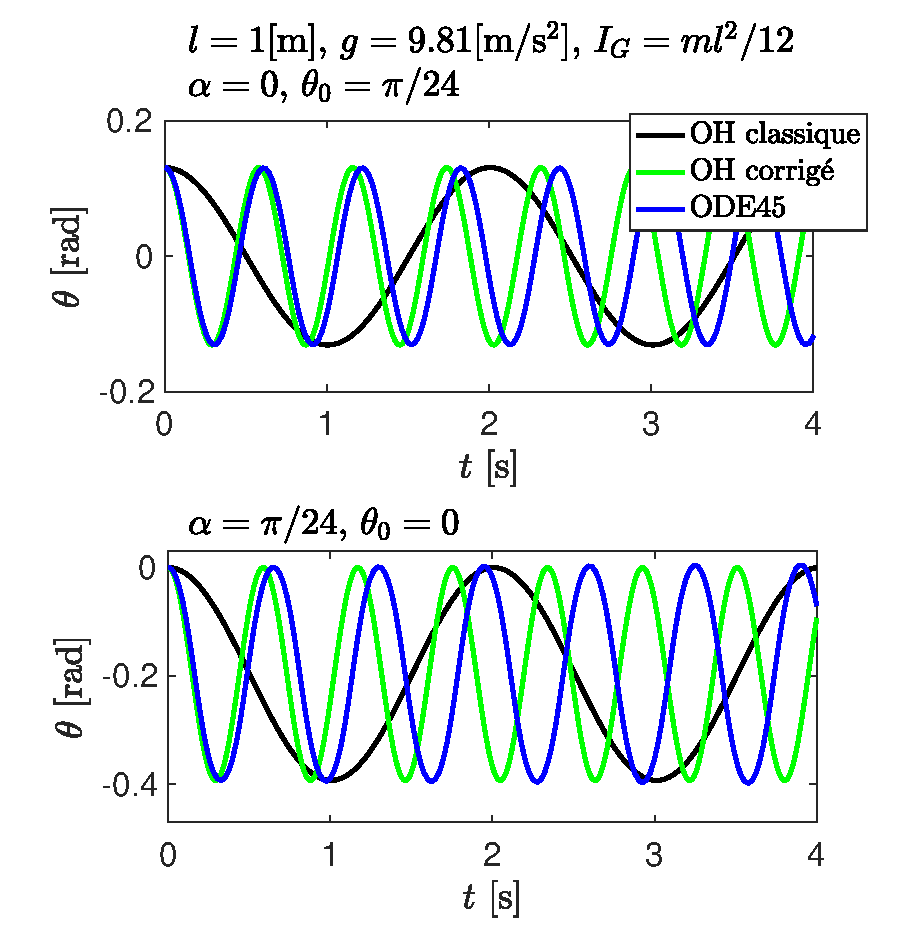
\includegraphics[width=0.95\linewidth]{ExoFig/tyr_solution_petites_oscillations.eps}
      \caption{Petites oscillations autour de l'équilibre.}
        \label{fig:solution_petites_oscillations}
    \end{subfigure}%
    \begin{subfigure}{.55\textwidth}
      \centering
        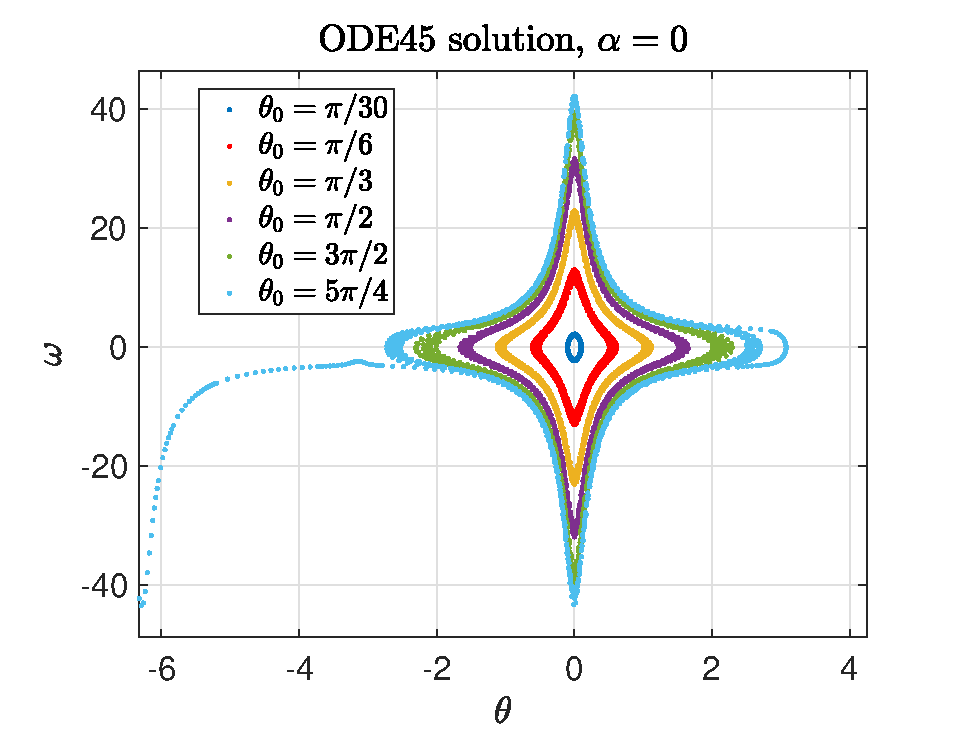
\includegraphics[width=0.95\linewidth]{ExoFig/tyr_solution_espace_de_phase.eps}
      \caption{Trajectoires dans l'espace de phase pour différentes conditions initiales.}
        \label{fig:espace_phase}
    \end{subfigure}
    \caption{Exemple de trajectoires calculées par \texttt{tyrolienne.m} et ODE45.N.B.: ces résultats utilisent un $\theta$ défini par rapport a la verticale et non par rapport a la perpendiculaire du câble. d'où les oscillations autour de $\theta=-\alpha$.}
    \label{fig:test}
    \end{figure}
%\end{solution}


%% PARTIE 2
\uplevel{On considère maintenant le cas $0<\alpha<\pi/2$. La tyrolienne est lâchée depuis le point $O$, perpendiculaire au câble et sans vitesse initiale, c'est-à-dire, à cet instant, $\theta=0$, $\dot\theta=0$ et $\dot x_{A}=0$.}

\part{Trouver une relation qui détermine l'angle maximal $\theta_{max}$ que la tyrolienne atteint en bout de course (lorsque $x_A=d$) en fonction des données du problème. 
Dans quelles conditions la tyrolienne parvient-elle à effectuer des rotations complètes autour du point $B$?}
%\begin{solution}
    \par\vspace{2mm}
    On procède par lois de conservation entre des instants clés.
    \subsubsection*{Instant $a$: condition initiale}
    L'énergie mécanique au point $O$, instant $a$ ($t=t_0$), est constituée uniquement d'énergie potentielle, i.e.
    \begin{equation}
        E_{a} =mgh
    \end{equation}
    avec $h=d\sin\alpha$ (on garde la lettre h jusqu'à la fin pour simplifier l'écriture). 
    Ici on a fixé le zéro de l'énergie potentielle lorsque la tyrolienne est au point $B$ a $\theta=0$.
    
    \subsubsection*{Instant $b$: juste avant le choc}
    Juste avant l'arrivée au point $B$, instant $b$, l'énergie potentielle est nulle et la tyrolienne ne tourne pas (position d'équilibre).
    L'énergie mécanique est donc égale à l'énergie cinétique de translation, i.e.
    \begin{equation}
        E_{b} = \frac{1}{2}mv_{G,b}^2.
    \end{equation}
    Entre les instants $a$ et $b$, L'énergie mécanique est conservée (il n'y a que la gravité qui travaille)
    \begin{equation}
        E_{a} = E_{b} \Leftrightarrow mgh = \frac{1}{2}mv_{G,b}^2,
    \end{equation}
    ce qui nous donne la vitesse du centre de masse (et de toute la tyrolienne par extension) à l'arrivée au point $B$, $v_{G,b}=\sqrt{2gh}$.
    Le moment cinétique au point $A$ à l'instant $b$ est donné par 
    \begin{equation}
        \bm L_{A,b} =\sum_i\overrightarrow{AP_i}\times m_i \bm v_{i,b} = \overrightarrow{AG}\times m \bm v_{G,b} + I_G \omega_b \ezACDH = ml\sqrt{2gh}\ezACDH,
    \end{equation}
    où $\omega_b=0$ car la barre n'effectue pas de rotation propre en cet instant.
    
    \subsubsection*{Instant $c$: juste après le choc}
    Lors de l'interaction avec le mécanisme au point $B$, la vitesse du point d'attache passe de $\dot x_{A}\exACDH =v_{G,b}\exACDH$ à $\dot x_{A}\exACDH =0$.
    Il y a donc une accélération non nulle du point d'attache ce qui implique l'existence d'une force $F_B\exACDH$ par la deuxième loi de Newton.
    Cette force travaille car elle est parallèle à la vitesse du point auquel elle s'applique.
    C'est pourquoi il n'y a ni conservation de l'énergie mécanique, ni conservation de la quantité de mouvement entre l'instant $b$ et $c$.
    Cependant, comme le moment de force associé à $\vec F_B$ est nul ($\vec M_B=\overrightarrow{AB}\times\vec F_B = 0$ car $\overrightarrow{AB}=0$), le moment cinétique au point $A$ est conservé lors du choc.
    Ainsi, juste après le choc, le moment cinétique au point $A$ s'écrit
    \begin{equation}
        \bm L_{A,c} =\overrightarrow{AG}\times m \bm v_{G,c} + I_G \omega_c \ezACDH = (1+\eta)mlv_{G,c}\ezACDH
    \end{equation}
    ou on a utilise $v_{G,c} =  l\omega_c$.
    On égalise maintenant le moment cinétique d'avant et d'après le choc pour obtenir la vitesse du centre de masse à l'instant $c$, i.e.
    \begin{equation}
        \bm L_{A,c} = \bm L_{A,b} \Leftrightarrow (1+\eta)mlv_{G,c} = ml\sqrt{2gh} \Leftrightarrow v_{G,c}= \frac{\sqrt{2gh}}{1+\eta}.
        \label{eq:mcin_A_c}
    \end{equation}
    L'énergie mécanique à l'instant $c$ est donnée par
    \begin{equation}
    E_{c} = \frac{1}{2}mv_{G,c}^2 + \frac{1}{2}I_G\omega_c^2 = \frac{1}{2}m\left(v_{G,c}^2 + \frac{I_G}{ml^2}v_{G,c}^2\right) = (1+\eta)\frac{1}{2}m v_{G,c}^2.
    \end{equation}
    
    \noteACDH{On peut vérifier que l'énergie mécanique n'est pas conservée en calculant sa variation entre l'instant $b$ et $c$
    $$
    E_{c} - E_{b} = (1+\eta)\frac{1}{2}m v_{G,c}^2 - \frac{1}{2}mv_{G,b}^2 =\left[(1+\eta) - (1+\eta)^2\right]\frac{1}{2}m v_{G,c}^2 = -\eta E_{c} = -\frac{\eta}{1+\eta}E_b < 0.
    $$
    Comme $\eta>0$ on en conclut que de l'énergie est absorbée par le mécanisme.
    La variation relative d'énergie est donnée par $\delta = |E_c-E_b|/E_b = \eta/(1+\eta)$. 
    Pour une barre homogène ($I_G = ml^2/48$) on obtient $\delta = 1/49$ alors que pour un pendule ($I_G=ml^2$) on a $\delta = 1/2$, i.e. $50\%$ de l'énergie initiale est absorbée dans le mécanisme.}
    
    \subsubsection*{Instant d: amplitude maximale}
    Quand l'amplitude maximale est atteinte, instant $d$, la tyrolienne ne tourne plus, $\omega_{d}=0$, donc l'énergie mécanique s'écrit
    \begin{equation}
        E_{d} = mgh_{max}
    \end{equation}
    L'énergie mécanique est conservée entre l'après choc ($c$) et l'amplitude maximale ($d$), on peut donc obtenir une equation pour $\theta_{max}$ en utilisant $h_{max}=l \cos(\alpha)-l\cos(\theta_{max}-\alpha)$, i.e.
    \begin{align}
        &(1+\eta)\frac{1}{2}mv_{G,c}^2 = mgh_{max} \nonumber\\
        \Leftrightarrow&\frac{mgh}{1+\eta} =mg l [\cos(\alpha)-\cos(\theta_{max}-\alpha)] \nonumber\\
        \Leftrightarrow&\cos(\theta_{max}-\alpha) = \cos(\alpha) - \frac{1}{1+\eta}\frac{h}{l}\nonumber\\
        \Leftrightarrow&\theta_{max}=\alpha+\arccos\left[\cos(\alpha) - \frac{1}{1+\eta}\frac{d}{l}\sin(\alpha)\right].
        \label{eq:ampmax}
    \end{align}
    Comme $-1\leq \cos \leq 1$, l'équation \eqref{eq:ampmax} ne possède pas toujours une solution.
    Ceci est lié au fait qu'au dessus d'une certaine hauteur de départ, la barre ne s'arrêtera pas et continuera de tourner indéfiniment autour du point $B$ selon notre modèle.
    L'angle limite vaut $\theta_{lim}=\alpha+\pi$ et donc la distance limite vaut
    \begin{align}
        d_{lim} = (1+\eta) \frac{\cos(\alpha) + 1}{\sin(\alpha)}l
        \label{eq:hlim}
    \end{align}
    Et donc la barre effectuera des tours sur elle même si $d>d_{lim}$.
    
    
    \noteACDH{Étudions quelques limites pour se convaincre du résultat.
    Si $\alpha=2n\pi$, $\sin\alpha=0$ et $\cos\alpha=1$ et donc $d_{lim}=\infty$ ce qui est logique car on est dans le cas d'un câble horizontal et les rotations complètes ne sont pas possible avec un angle de départ nul.
    Si $\alpha=(2n+1)\pi$, $\sin\alpha=0$ et $\cos\alpha=-1$ et donc $d_{lim}="0/0"$.
    On calcule cette limite avec le théorème de l'Hospital et on obtient  $d_{lim}=0$ ce qui est logique car on est dans le cas "retourné" où la tyrolienne est au dessus du câble.
    Pour $\alpha =\pi/2$ on a $d_{lim}=(1+\eta)l$ ce qui donne $d_{lim}=2l$ dans le cas d'un pendule ($\eta = 1$). 
    Ce résultat coïncide avec le résultat sur le $\delta$ d'énergie mécanique absorbée par le mécanisme qui prédisait une perte de $50\%$ d'énergie initiale. }
%\end{solution}

\end{parts}
\end{document}